\documentclass[11pt]{article}
%\documentclass[a4paper,11pt]{scrartcl}
\usepackage{amsmath} 
\usepackage{fullpage}
\usepackage[utf8]{inputenc}
\usepackage{graphicx}
\usepackage{listings}
\usepackage{color}


%--------Meta Data: Fill in your info------

\begin{document}

\section{Understanding the VARCode}
The code folder structure should be as follows:
\begin{itemize}
\item[1)] VarCode
  \begin{itemize}
  \item[a.] Code $\rightarrow$ this folder contains the code to run the VAR,
  \item[b.] Data $\rightarrow$ this folder contains the data run in the VAR,
  \item[c.] Outdata $\rightarrow$ this folder contains the output of the VAR,
  \item[d.] Documentation $\rightarrow$ this folder contains the documentation to the code (this file you're reading right now!).
  \end{itemize}
\end{itemize}

\subsection{Code}
The following folder contains two files, the \textit{main.jl} file which is the only one that you need to run in julia by opening Julia-0.5 and running the command: $$\text{\textit{include(``main.jl'')}}.$$

The second file, \textit{option.jl} is the only file you need to modify in the Code folder in order to run whatever version of the VAR you wish to run. Here are the options:
\begin{itemize}
\item[VAR options:]
  \begin{itemize}
  \item p: number of lags for the VAR,
  \item date\_format: format the dates in the $.csv$ file are in (e.g. "yyyy-mm-dd"),
  \item start\_date: the date you wish the VAR to start (remember that if you are using differences then you lose one period!),
  \item end\_date: the date you wish the VAR to end,
  \item Vars: the names you wish the code to use for the variables you are including in the VAR (be consistent with the order across \textit{Vars}, \textit{Mnems}, \textit{Vars\_names} and \textit{Transformations}),
  \item Mnems: the mnemonics that these variables have in your \textit{.csv} sheet (necessary for identification of the columns),
  \item Vars\_names: the full names of the series as you wish they appear in plot titles,
  \item Transformations: transformations applied to each series (in order),
  \item dates\_mnems: mnemonic for the date column,
  \end{itemize}
\item[IRF options:]
  \begin{itemize}
  \item ndraws: number of draws to compute the confidence intervals of the IRFs,
  \item nperiods: number of periods to show in IRF plot
  \item conf\_int: size of confidence interval (e.g. 90\%, 70\%, etc).
  \end{itemize}

Furthermore, the folder contains a subfolder called ``functions'' which contains functions used by the main file. These need not be touched but can be modified ad hoc. The functions are:

\begin{itemize}
  \item[Data\_organizer:] This function takes in the data as a dataframe, the mnemonics, the start line and the end line (corresponding to the start\_date and end\_date), the transformations for each series as well as the number of periods and number of variables. It uses these inputs to create a matrix of the data where each row corresponds to the data series specified in the option file.
  \item[var\_reg:] This function runs the VAR in OLS form and spits out the estimated coefficients, the estimated variance of the residuals, the fits, the actual (dependent data, i.e. LHS of regression) and the independent variables (RHS of regression).
  \item[forecast:] This function does the $h$-period ahead forecast of the variables with the VAR, where $h$ is indicated by the user ($h=1$ in $main.jl$).
  \item[imp\_res:] This function, given the estimated VAR outputs, gives a 4-dimensional matrix with the IRF data (nperiods$\times$n$\times$n$\times$ndraws), where the second $n$ indicates the response and the third indicates the shock.
  \item[RMSE:] Computes the RMSE given the Actual and the Fit.
  \item[dummy\_fores:] Computes fake data based on the ``initial data'' (i.e. the first p periods of the data necessary to forecast). The ``dummy data'' is a necessary part of the boot-strapping used to get confidence intervals.
\end{itemize}

\end{itemize}


\subsection{Data}
The data folder only contains the data file which, by default, is called \textit{Data.csv}. This file should be a \textit{.csv} file and should contain the dates (with some column title) and each series with their respective (unique) titles.

It is important to give it this structure so that the program is capable of reading the table correctly and structuring the VAR properly.


\subsection{Outdata}
This folder contains the following sub-folders:

\begin{itemize}
  \item[IRFs:] Here you will find all the impulse response functions named using the following convention: \textit{IRF\_shockvar\_responsevar.pdf}.
\end{itemize}


\clearpage

\section{Some Theory}

\subsection{Estimating the VAR}

The way we estimated the VAR is by constructing first the LHS and the RHS variables given all data available $$\underset{T\times n}{Y_{1:T}} = \begin{pmatrix}
y_{1,1} & y_{1,2} & \cdots & y_{1,n}\\
\cdots & \cdots & \cdots & \cdots\\
y_{T,1} & y_{T,2} & \cdots & y_{T,n}\\
\end{pmatrix}$$

The model will then look like:

$$LHS = RHS\cdot \beta,$$

where

$$\underset{(T-p)\times n}{LHS} = \begin{pmatrix}
y_{p+1,1} & y_{p+1,2} & \cdots & y_{p+1,n}\\
\cdots & \cdots & \cdots & \cdots\\
y_{T,1} & y_{T,2} & \cdots & y_{T,n}
\end{pmatrix}$$

and 

$$\underset{(T-p)\times np}{RHS} = \begin{pmatrix}
y_{p,1} &  \cdots & y_{p,n} &  \cdots &  \cdots &  y_{1,1}  & \cdots & y_{1,n}\\
\cdots &  \cdots & \cdots & \cdots &  \cdots &  \cdots & \cdots & \cdots \\
y_{T-1,1} &  \cdots & y_{T-1,n} &  \cdots  &  \cdots  & y_{T-p,1} & \cdots & y_{T-p,n}
\end{pmatrix}$$


As we include a constant term (which the code does) our RHS will be augmented as follows,

$$\underset{(T-p)\times (np+1)}{RHS} = \begin{pmatrix}
1 & y_{p,1} &  \cdots & y_{p,n} &  \cdots &  \cdots &  y_{1,1}  & \cdots & y_{1,n}\\
1 & \cdots &  \cdots & \cdots & \cdots &  \cdots &  \cdots & \cdots & \cdots \\
1 & y_{T-1,1} &  \cdots & y_{T-1,n} &  \cdots  &  \cdots  & y_{T-p,1} & \cdots & y_{T-p,n}
\end{pmatrix}$$

This brings us to the estimation (in simple OLS form): 
\begin{equation}\label{1}
\underset{(np +1)\times n}{\hat{\beta}} = (\underset{(np+1)\times (T-p)}{RHS'}\cdot \underset{(T-p)\times (np+1)}{RHS})^{-1}\cdot \underset{(np+1) \times (T-p)}{RHS'}\cdot \underset{(T-p)\times n}{LHS}
\end{equation}

and 
\begin{equation}
\underset{n\times n}{\hat{\Sigma}} = \frac{(LHS-RHS \times \hat{\beta})'*(LHS-RHS \times \hat{\beta})}{T}
\end{equation}

Furthermore, assuming that the regression has been run with a constant term, we can re-organize $\hat{\beta}$ as 
\begin{equation}
\underset{np\times 1}{C} = \begin{pmatrix} \hat{\beta}[1,:]'\\ 0_{(p-1)*n\times 1} \end{pmatrix}
\end{equation}
 containing the constant term, and 
\begin{equation}\underset{np\times np}{\Psi} = \begin{pmatrix} \hat{\beta}[2:end,:]'\\
[I_{(p-1)\cdot n \times (p-1)\cdot n} 0_{(p-1)\cdot n,n}] \end{pmatrix}
\end{equation}

which allows us to write the VAR in companion form $$\underset{np\times 1}{Z_{t}} = \underset{np\times 1}{C} + \underset{np\times np}{\Psi}\cdot \underset{np\times 1}{Z_{t-1}} + \underset{np\times 1}{\vec{\epsilon}_{t}}$$
where $Z_{t} = \begin{pmatrix}z_{t}\\ z_{t-1}\\ \cdot \\ z_{t-p+1}\end{pmatrix}$, 
$z_{t} = \begin{pmatrix}
  y_{1,t}\\
  \cdot\\
  y_{n,t}\\
\end{pmatrix}$
  and $\vec{\epsilon}_{t} = \begin{pmatrix} \epsilon_{t}\\ 0_{n(p-1) \times 1} \end{pmatrix}$, with 
$\epsilon_{t} = \begin{pmatrix}
  \varepsilon_{1,t}\\
  \cdots \\
  \varepsilon_{4,t}\\
\end{pmatrix}$ in particular $\vec{\epsilon}_{t}\sim \mathcal{N} \Big(0,\begin{pmatrix} \Sigma & 0\\ 0 & 0 \end{pmatrix} \Big)$



\subsection{Forecast}

We derive the equation used for our forecasting applying recursively the following $$ Z_{t+1|t} = E[C+\Psi Z_{t} + \epsilon_{t}] = C+\Psi Z_{t}$$ 
\begin{align*}
 Z_{t+h|t} &= C+ \Psi Z_{t+h-1|t} =C + \Psi (C+\Psi Z_{t+h-2|t}) \\ 
&=\cdots \\
&= (\underset{j=0}{\overset{h-1}{\sum}}{\Psi}^{j})C + {\Psi}^{h} Z_{t}
\end{align*}

\subsection{Impulse Response Functions}

The aim here is, for h=1:H, to get $\frac{\partial Y_{t+h}}{\partial \epsilon_{t,j}}$, i.e. looking at how the vector of variables at times $t+h$ respond to a shock of variable $j$ at time $t$.

Our system can be written as above (using the explicit form of eq. 4):

$$\begin{pmatrix}
   z_{t}\\
   \cdot\\
   z_{t-p+1}
  \end{pmatrix} = C + 
  \begin{pmatrix} A_{1} & \cdots & A_{p}\\
  I_{(p-1)\cdot n \times (p-1)\cdot n} & \cdots & O_{(p-1)\cdot n\times n} \end{pmatrix} \begin{pmatrix}
   z_{t-1}\\
   \cdot\\
   z_{t-p}
  \end{pmatrix} + \begin{pmatrix}
   \epsilon_{t}\\
   O_{n(p-1) \times 1}
  \end{pmatrix}$$

Renaming appropriately, this system can be written as 
$$ Z_{t} = C + \Psi Z_{t-1} + S' \epsilon_{t}$$

where $S = \begin{pmatrix} I_{n\times n} O_{n\times n(p-1)} \end{pmatrix}$.

Because the shocks are not necessarily orthogonal, we use the Cholesky decomposition $Pu_{t} = \epsilon_{t}$ where $P = chol(\hat{\Sigma})$ (lower-triangular). Thus we have

$Z_{t+1} = C+ \Psi(C+ \Psi Z_{t-1} + S' P u_{t}) + S'Pu_{t+1}$, $Z_{t+2} = C + \Psi(C+ \Psi(C+ \Psi Z_{t-1} + S' P u_{t}) + S'Pu_{t+1}) + S'Pu_{t+2}$. However, once we take the partial with respect to $u_{t}$ we notice that all terms except for $u_{t}$ do not matter. Thus we have

\begin{align*}
\frac{\partial Z_{t+h}}{\partial u_{t}} &= \frac{\partial Z_{t+h}}{\partial u_{t}} = \Psi^{h}\cdot S' \cdot P 
\end{align*}

If we want to select the response at a certain time $t'$ we then pre-multiply this result by the appropriate selection matrix. For example, to select the response on the latest period $t+h$ we pre-multiply by $S$.
\clearpage



\section{An example}

Included in this folder is an example used for a weekly briefing. 

We run a VAR with three variables: unemployment rate (UNRATE), housing starts (HSN1F) and industrial production (INDPRO). Notice, both the names you want the variables to be called and the mnemonics of reference in the \textit{Data.csv} need to be inputted in the data file. Furthermore, the data contains also a date column whose name needs to be specified (in this case it is observation\_date).

Since we want the series to be in level for all three series, we include these transformations in the \textit{options.jl} file as `lvl'. 

We run the main file opening julia in the terminal as follows (this will look different from different terminals):

\vspace*{1em}
\begin{center}
\begin{figure}[ht!]
    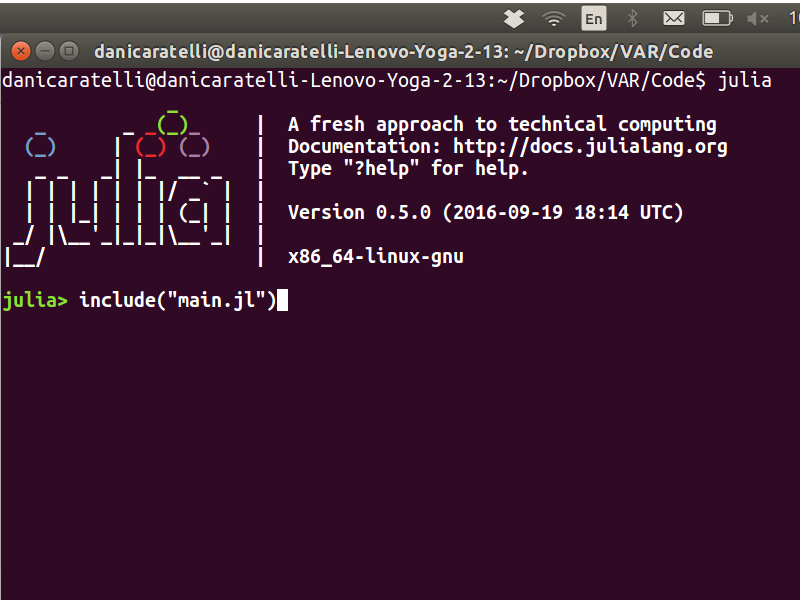
\includegraphics[scale=0.4, trim={0cm 0cm 0cm 1cm},clip]{terminal_view.png}\\
\end{figure}
\end{center}
\vspace*{1em}


This will produce IRF plots contained in the appropriate folder such as the following:\\

\vspace*{-1em}
\begin{center}
\begin{figure}[ht!]
    \includegraphics[scale=1, trim={0cm 0cm 0cm 0cm},clip]{../Outdata/IRFs/IRF_houses_houses.pdf}\\
    \includegraphics[scale=1, trim={0cm 0cm 0cm 0cm},clip]{../Outdata/IRFs/IRF_houses_ip.pdf}\\
    \includegraphics[scale=1, trim={0cm 0cm 0cm 0cm},clip]{../Outdata/IRFs/IRF_houses_u3.pdf}\\
\end{figure}
\end{center}


\end{document}